\section{寄存器描述}
\regover{
{\hyperref[cks-cks-config]{cks\_config}}&
\\
\hline
{\hyperref[cks-data-in]{data\_in}}&
\\
\hline
{\hyperref[cks-cks-out]{cks\_out}}&
\\
\hline
}

\subsection{cks\_config}
\label{cks-cks-config}
地址:0x2000a700
 \begin{figure}[H]
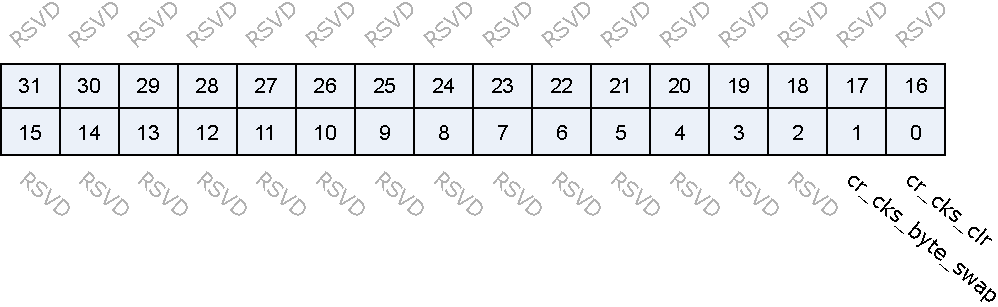
\includegraphics{cks_cks_config.pdf}
\end{figure}

\regdes{31:2&RSVD& & & \\\hline
1&cr\_cks\_byte\_swap&r/w&1'b0&Byte swap signal for each 16-bit data \par 1'b0: The first data pushed should be the upper byte \par 1'b1: The first data pushed should be the lower byte
\\\hline
0&cr\_cks\_clr&w1c&1'b0&Checksum clear (reset) signal\\\hline

}
\subsection{data\_in}
\label{cks-data-in}
地址:0x2000a704
 \begin{figure}[H]
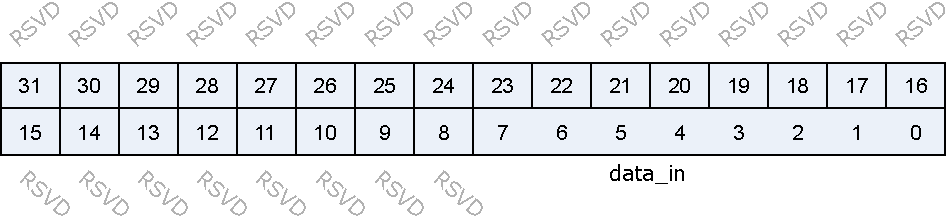
\includegraphics{cks_data_in.pdf}
\end{figure}

\regdes{31:8&RSVD& & & \\\hline
7:0&data\_in&w&x&Data input\\\hline

}
\subsection{cks\_out}
\label{cks-cks-out}
地址:0x2000a708
 \begin{figure}[H]
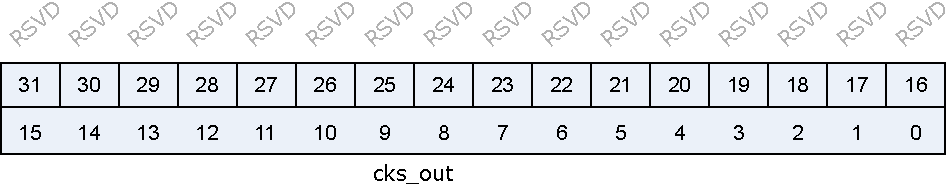
\includegraphics{cks_cks_out.pdf}
\end{figure}

\regdes{31:16&RSVD& & & \\\hline
15:0&cks\_out&r&16'hFFFF&Checksum output\\\hline

}
